\chapter{Digital Communication}
This first section is all about how to convert and transmit some signal.\
\begin{section}{Introduction}
The goal of communication is to transmit some kind of data form a sender to a receiver. In order 
to do so, the physical layer defines the means of transmitting a stream of \textbf{raw bits} over a
physical data link, which connects those two nodes.\\
Data is transmitted in the form of \textbf{signals}, which are a physical representation of the data.
The signal is transmitted over a \textbf{channel}, which is the transmission medium that connects 
the sender and receiver. This can be both wired or wireless.\\
Whereas with wired channels, checking the device connected to the channel is easier to implement, 
with wireless ones security is a major when travelling in the channel. This is for may reasons:
\begin{itemize}
  \item No inherent protection is applied to the channel( it is replaced by a logical association)
     \subitem sending and receiving messages do not need physical access to the network 
     infrastructure
  \item the communication is in broadcast, which is intrinsic of radio nature.
    \subitem Transmission can be overheard by anyone in range( which can be quite big, depending 
    on the situation), and anyone can generate a transmission, for example by jamming nearby 
    transmissions.
\end{itemize}
As a result:
\begin{itemize}
  \item Eavesdropping is easy
  \item Injecting fake messages into the communication in easy
  \item replaying previously recorded messages is easy(\textit{meaconing}). This is actually very 
    dangerous for gps positioning, so it is also a security concern.
  \item illegitimate access to the network and its services is easy
  \item Denial of service attacks are easy, achieved by jamming the channel.
\end{itemize}
% 9/43
\end{section}
\begin{section}{Digital Communication System}
The digital communication system in characterized by three sections: 

\begin{itemize}
  \item the \textbf{user section}, which consist in the transmitter and the receiver, that want to 
    communicate. 
  \item the \textbf{interface section}, which is the interface to conveying the signal from the 
    user to the analog channel. It also transforms bits to analog signal, compressing and encoding 
    them, also associating bits to signal waveforms, to transform bits to analog signal.
  \item the \textbf{channel section}, which is the physical medium, that can only propagate analog 
    waveforms. In the end, we want to transmit digital signal but we are forced to use analog ones.
\end{itemize}

\begin{figure}[h]
  \centering
  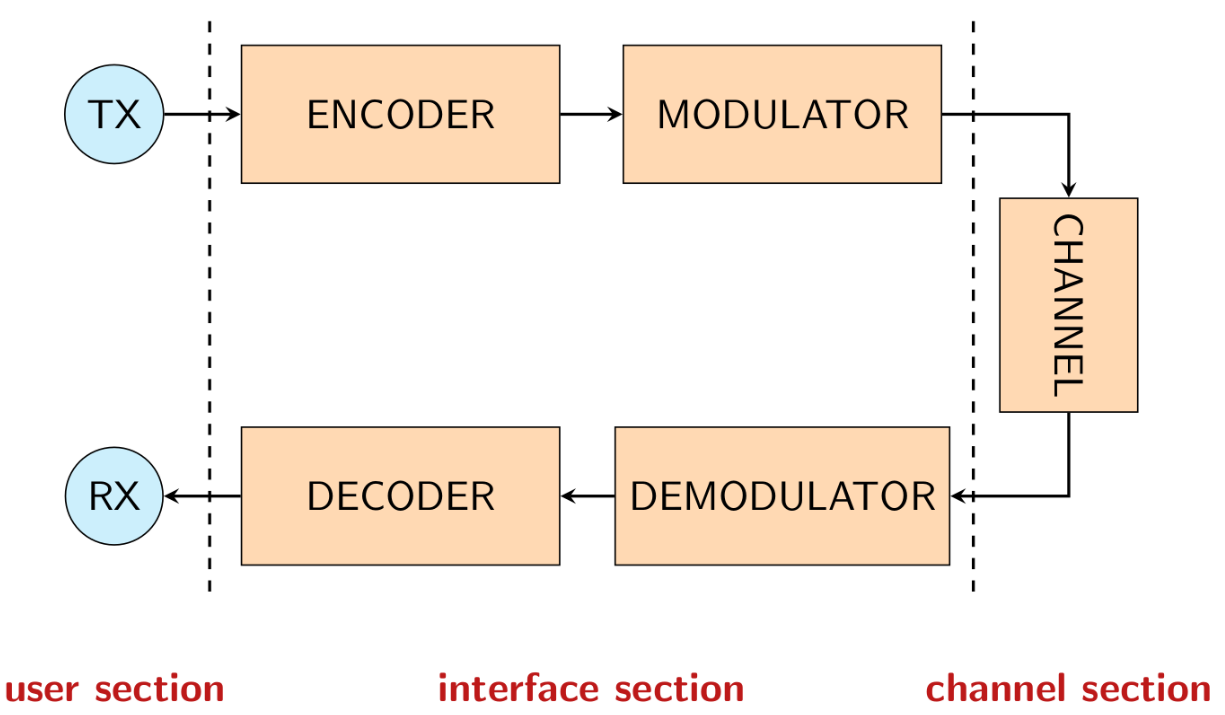
\includegraphics[width=0.7\textwidth]{img/digital communication schema.png}
  \caption{Digital Communication System}
  \label{fig:Digital Communication System}
\end{figure}
\begin{subsection}{The transmitter chain}
The transmitter chain is the part of the system that takes the digital signal, or an analog one 
converted to digital, and converts it to an analog signal, that can be transmitted over the
channel.\\
It is basically composed by two parts. The first one being an \textbf{encoder}, which can limit the amount 
of bits transmitted(\textit{source encoding}), and/or make the transmitted sequence more robust to
errors(\textit{channel encoding}).\\
The second one is the \textbf{modulator}, which is the part of the system that takes the digital
signal and converts it to an analog one to transmit it over the channel.
\end{subsection}
\begin{subsection}{The channel}
The channel is the physical medium that transfers bits from interface to interface, from the sender
to the receiver.
Its operation is affected by different types of disturbances such as:
\begin{itemize}
	\item frequency-domain distortion
	\item wireless fading
	\item additive noise
	\item impulsive noise
	\item interference from other frequency channels (interchannel interference)
	\item interference from the same frequency channel (cochannel interference)
	\item Intentional interference
\end {itemize}
\end{subsection}
\begin{subsection}{The receiver chain}
The receiver chain is the part of the system that takes the analog signal from the channel and
converts it to a digital signal, that can be processed by the user.\\
It is composed by the dual counterpart of the transmitter chain, the \textbf{demodulator} and the
\textbf{decoder}. \\
The demodulator takes the analog signal and converts it to a sequence of samples that can be
processed by the decoder.\\
The decoder takes the sequence of samples and converts it to a digital signal. It implements
\textit{channel decoding}, to correct errors, and \textit{source decoding}, to recover the original
message.
\end{subsection}
\end{section}

\begin{section}{Signal representation and Processing}
  \begin{boxH}
    A \textbf{signal} is a (mathematical) function that conveys information about a phenomenon.
  \end{boxH}
  Basically, any quantity that varies over space or time can be used to represent a informations,
  allowing to describe the evolution of physical quantities over time(voltages, currents, \dots).\\
  Its mathematical representation is therefore a function of real variable (time) taking real or 
  complex(more than one) values.\\
  We will be mostly focused on Electromagnetic Signals (e.g. voltage), but the general concepts 
  can be applied to any kind of signal
  \begin{subsection}{Energy of a signal}
    The energy of a signal is the integral of the squared modulus of the signal itself.
    \begin{equation}
      E(x) = \int_{-\infty}^{\infty} |x(t)|^2 dt
    \end{equation}
    As we can see , the energy is a scalar value, and the whole function is made positive by the
    squared modulus.\\
    \begin{figure}[h]
      \centering
      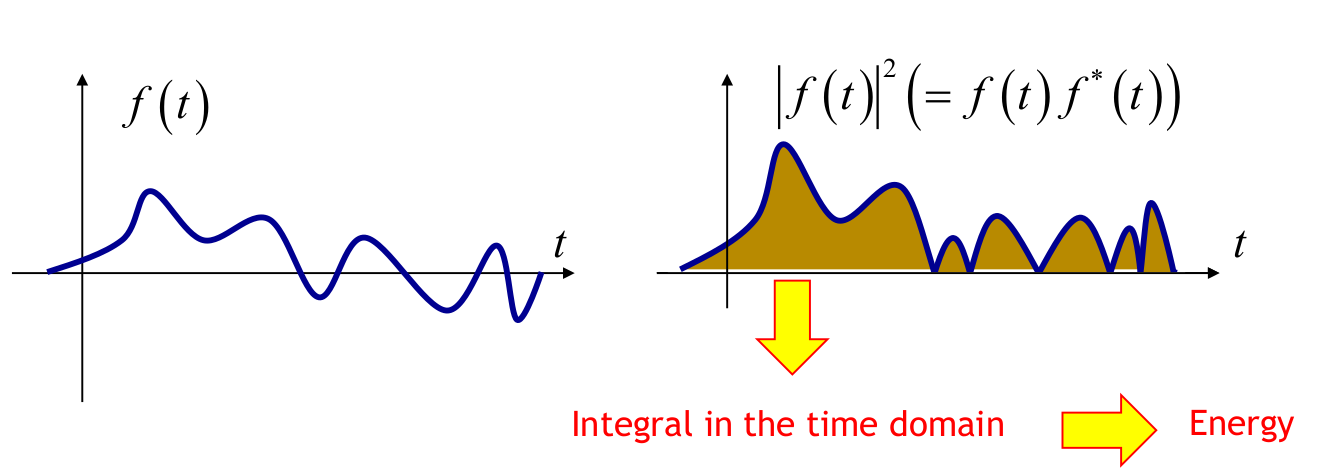
\includegraphics[width=0.7\textwidth]{img/energy signal.png}
      \caption{Energy of a signal}
      \label{fig:Energy of a signal}
    \end{figure}
    A signal with a very large amplitude, over time, will have a very high energy, while a signal
    which assumes values close to zero will have a very low energy, being a very weak signal.\\
    Furthermore, we can note that the more distant is the signal from the origin, the larger the energy.
  \end{subsection}
  \begin{subsection}{Power of a signal}
    When we refer to power we can refer to the \textbf{instantaneous power} of a signal, which is just the 
    square module of a signal
    \begin{equation}
      P(x) = |x(t)|^2
    \end{equation}
    but much more commonly we refer to the average power of a signal, which is the time average of
    the instantaneous power of the whole signal.
    \begin{equation}
      P(x) = \lim_{a \to \infty} \frac{1}{2a} \int_{-a}^{a} |x(t)|^2 dt
    \end{equation}
    This a again a scalar value.
  \end{subsection}
  \begin{subsection}{Signal Representation}
    To analyze and process the signals, it is necessary to adequately represent them, and the
    definition of signals as "time functions" is NOT effective for many applications, for many 
    reasons.\\
    Generally, signals can become very complicated depending on our communication system, and
    we want different ways of representing them, to make them easier to process.\\
    For instance, we can represent a signal as a sum of elementary signals, thanks to the scalar
    product of the signal with a basis of the space of signals.\\

    The scalar product between signals is a scalar value, which is a measure of the similarity 
    among signals.\\
    If two function are quite similar we will get a large number.
    It it is zero, they are said to be orthogonal.
    \begin{equation}
      \langle x,y \rangle = \langle x(t),y(t) \rangle = \int_{-\infty}^{\infty} x(t)y^*(t) dt
    \end{equation}

    So, if we have a set of elementary signals $w_1(t), w_2(t), \dots, w_m(t)$, we write the signal
    $x(t)$ as a linear combination of the elementary signals:
    \begin{equation}
      x(t) = \sum_{i=1}^{m} \alpha_i w_i(t)
    \end{equation}
    where $\alpha_i$ are the coefficients of the linear combination $\alpha_i = \langle x(t), 
    w_i(t) \rangle$.\\
    In a more down to hearth way, the coefficient $\alpha_i$ allows us to understand how much each
    individual signal is similar to any other elementary signal we are considering, and because the 
    scalar product is higher for similar signals, we can understand how much each elementary signal
    is contributing to the whole signal.\\

    Furthermore, by adjusting the coefficient, we are able to create a whole different signal using
    the same elementary signals.
    \begin{subsubsection}{A common example: In Phase and Quadrature components representation}
      Lets consider a very simple basis, or a set of elementary signals, which is actually more 
      important that many other ones:
      \begin{itemize}
        \item the \textbf{in-phase} signal, which is a cosine function $w_1(t) = cos(2\pi f_o t)$
        \item the \textbf{quadrature} signal, which is a sine function $w_2(t) = sin(2\pi f_o t)$
      \end{itemize}
      where $f_o$ is the frequency, in Hz, of the signal.\\
      We can write any signal as a linear combination of these two signals, just by adjusting the
      coefficients:
      \begin{equation}
        x(t) = x_1 cos(2\pi f_o t) + x_2 sin(2\pi f_o t)
      \end{equation}
      where x(t) is the signal we want to represent, and $x_1$ and $x_2$ are the coefficients of the
      linear combination.\\

      A very simple representation of this complex signal is obtainable by representing each signal 
      as an axes in a complex plane, for example in figure \ref{fig:Complex Plane} the x-axis 
      is the in-phase signal, and the y-axis is the quadrature signal.\\
      Each signal can be represented as a point in the complex plane, because the distance from the
      origin signal(\textit{axis}) is the amplitude of the signal.
      For example, choosing a point close to the x-axis, we are choosing a signal with a very low
      quadrature component, and a very high in-phase component.Furthermore, a set of those 
      different points is called a \textit{constellation}\\
      \begin{figure}[h]
        \centering
        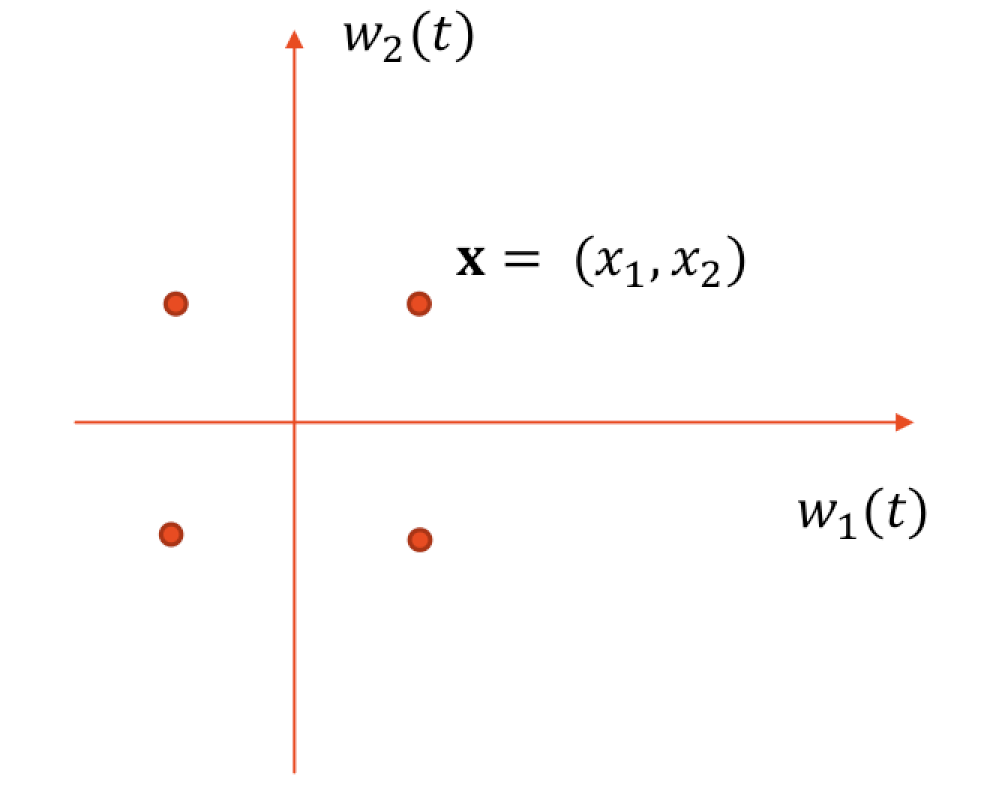
\includegraphics[width=0.5\textwidth]{img/iq representation.png}
        \caption{Some points that represent some signals in the I/Q representation}
        \label{fig:Complex Plane}
      \end{figure}
    \end{subsubsection}
  \end{subsection}
  \begin{subsection}{Fourier Analysis}
    Lets consider a signal with base the complex exponential functions 
    \begin{equation}
      e^{j2\pi \frac{n}{T} t} = cos(2\pi \frac{n}{T} t) + j sin(2\pi \frac{n}{T} t)
      \label{euler formula}
    \end{equation}
    It is actually characterized by a frequency $f_n = \frac{n}{T}$, where T is the period of the
    signal. The higher the frequency, the more oscillations we will have in the same time interval.
    In this function they have both the same frequency.\\

    We can use that function as a basis to decompose a signal, again. This is because it is 
    possible to generate an infinite set of functions
    \begin{equation}
      w_n(t) = \frac{1}{\sqrt{T}} e^{j\frac{2\pi}{T} nt} 
    \end{equation}
    with $-T/2 \leq t \leq T/2$, each associated with a frequency.
    That can be used ad a complete basis for all the signals limited in $[-T/2, T/2]$ or periodic.\\
    For example, we can write a signal as a linear combination of these functions:
    \begin{equation}
      x(t) = \frac{1}{\sqrt{T}} \sum_{n=-\infty}^{\infty} c_n e^{j\frac{2\pi}{T} nt}
      \label{Fourier Series}
    \end{equation}
    where $c_n$ are the coefficients of the linear combination $c_n = \langle x(t), w_n(t) \rangle$.\\
    Each one of those coefficients is a measure of how much each frequency $f_n$, of the $n$-th
    sinusoid(the shape of equation \ref{euler formula}) is present in the signal $x(t)$.\\
    \begin{figure}[h]
      \centering
      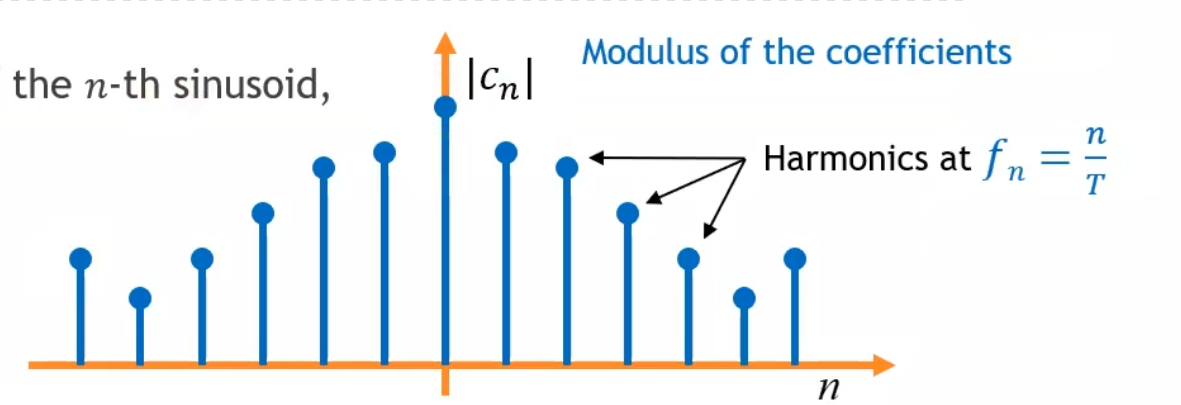
\includegraphics[width=0.7\textwidth]{img/euler plot.png}
      \caption{Plot of the coefficients of equation \ref{Fourier Series}}
      \label{fig:Fourier Analysis}
    \end{figure}
    Lets now take a look at picture \ref{fig:Fourier Analysis}. We can see that the coefficients
    are higher when the frequence is very small, so the signal \ref{Fourier Series} is mostly
    composed by large components of low frequency.\\
    This whole concept is called \textbf{Fourier Analysis}, or frequency analysis, which allows
    to decompose a signal into a set of frequencies.
    \begin{boxH}
    TLDR: I can build a signal trough a combination of frequency components. \\
    The coefficients of this frequency components are the measure of how much each frequency is 
    present in the signal.
    \end{boxH}
    Now we just need to expand it to any signal and any frequency( a continuous frequency domain).
    By doing so we can derive the definition of the \textbf{Fourier Transform} of a signal $x(t)$:
    \begin{equation}
      X(f) = \int_{-\infty}^{\infty} x(t) e^{-j2\pi ft} dt
      \label{Fourier Transform}
    \end{equation}
    where $X(f)$ is the Fourier Transform of the signal $x(t)$, and $f$ is the frequency.\\
    The Fourier transform is equivalent to a scalar product between the signal and the complex
    exponential function at a given frequency $f$. This means that each of the values of the
    Fourier Transform is a measure of how much the frequency $f$ is present in the signal $x(t)$.\\
    Furthermore, trough the inverse of equation \ref{Fourier Transform}
    \begin{equation}
      x(t) = \int_{-\infty}^{\infty} X(f) e^{j2\pi ft} df
      \label{Inverse Fourier Transform}
    \end{equation}
    we can write again a signal $x(t)$ as a linear combination of the complex exponential functions
    , which represents the frequency components of the signal, weighted by the Fourier Transform.\\
      
    \begin{boxH}
      The Fourier Transform $X(F)$ indicates the "weight" of each frequency component( sinusoidal
      component at a given frequency $f$) in the signal $x(t)$.\\
      The inverse Fourier Transform $x(t)$ tells us we can decompose any signal into frequency 
      components( sinusoidal components at a given frequency $f$).
    \end{boxH}
    
    \begin{figure}[h]
      \centering
      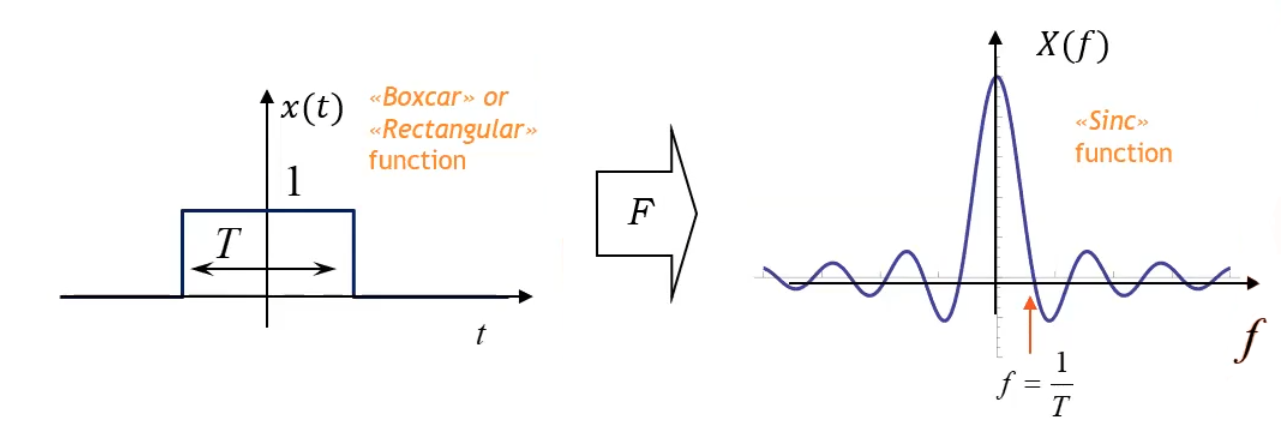
\includegraphics[width=0.9\textwidth]{img/fourier square function.png}
      \caption{Fourier Transform of a square function}
      \label{fig:Fourier Transform}
    \end{figure}

    With that in mind, take a look at figure \ref{fig:Fourier Transform}. It represents a rectangular
    signal (a signal that is 1 for a certain time, and 0 for the rest of the time), and its Fourier
    Transform, which tells us the frequency components of the signal.\\
    From that, we can see that the Fourier Transform is mostly composed by low frequency components,
    because values closer to zero are higher. That is because in the constant part of the signal
    has a sinusoidal component that constant.

    \begin{boxH}
      To wrap it up, for each signal we have a \textbf{spectral representation}. And for each operation
      over a signal, there are equivalents effects in the frequency domain.\\
      Furthermore, a signal that has finite duration in time, has a infinite support in the frequency
      domain.
    \end{boxH}
  \end{subsection}
  \begin{subsection}{Bandwidth}
    The bandwidth is the \textbf{interval of frequencies} that a signal occupies.\\
    If we consider a signal $x(t)$, we can define the bandwidth as the interval of frequencies
    where the Fourier Transform $X(f)$ is different from zero. \\ 
    Signals have often infinite support over the frequency domain over a finite duration, but many 
    of them are characterized by a quasi-null(finite) spectrum outside a certain interval of 
    frequencies( the main lobes of the spectrum).\\
    For this reason, we usually consider the bandwidth around half of the frequency spectrum of the
    signal, as shown in figure \ref{fig:Bandwidth}(for example 3dB bandwidth, or half power 
    bandwidth).\\
    \begin{figure}[h]
      \centering
      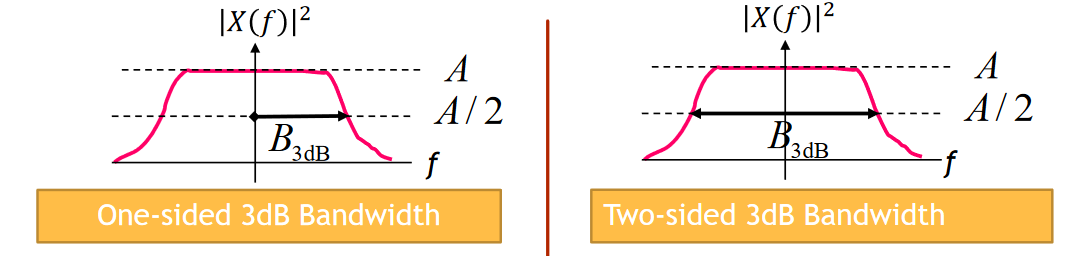
\includegraphics[width=0.8\textwidth]{img/bandwidth.png}
      \caption{Bandwidth of a signal}
      \label{fig:Bandwidth}
    \end{figure}
    \begin{subsubsection}{Bandwidth in linear systems}
      A \textbf{system} is a set of operations applied to signals.\\
      The relationship between the bandwidth of the input signal and the bandwidth of a system is
      usually very important. In fact, when a system is used to pass or remove particular 
      frequencies of a signal, it can be regarded as a system.\\
      We can associate a bandwidth to a system, specifically a \textbf{linear-time invariant} system,
      with a \textbf{frequency response} $H(f)$.This mean that we can associate a bandwidth to a
      system, making us able to compute a new bandwidth $Y(f)$ by combining together the bandwidth 
      $X(f)$ of the input signal and the frequency response $H(f)$ of the system($Y(f) = X(f)H(f)$
      in formulas).\\
      This concept can be represented graphically very easily, like in figure 
      \ref{fig:Bandwidth System}. If the result of the combination of the input signal and the
      sequence of operation of the system is a signal with a bandwidth $Y(f)$. If the bandwidth of 
      the linear system is larger than the origin signal, the signal pass trough smoothly($Y(f) \approx X(f)$).\\
      However, if the bandwidth of the signal is larger than the bandwidth of the system, the signal
      will be cutted off($Y(f) \ne H(f)$).\\

      \begin{figure}[h]
        \centering
        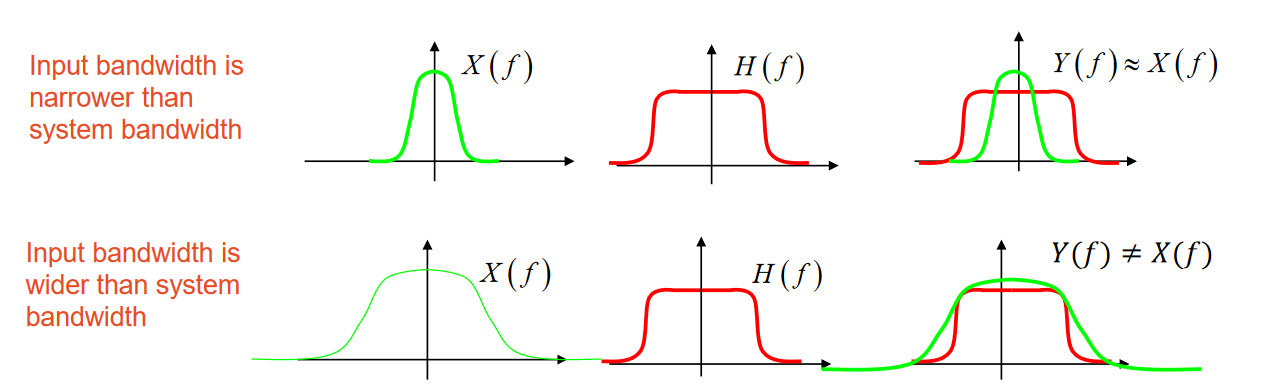
\includegraphics[width=0.8\textwidth]{img/bandwidth system.png}
        \caption{Bandwidth of a system}
        \label{fig:Bandwidth System}
      \end{figure}
    \end{subsubsection}
  \end{subsection}

  \begin{subsection}{Filters}
    A filter is a system used to model desired and undesired effects over a signal.\\
    It is usually used to remove undesired frequency components from a signal, but overall can be
    used to:
    \begin{itemize}
      \item share the wireless medium
      \item model the spectrum of a signal over the channel
      \item mitigate undesired effects over a signal trough equalizers
    \end{itemize}
    \end{subsection}
    \begin{subsection}{Signal modulation}
      Signal modulation is the process of multiplying a signal by a sinusoidal function, resulting
      in a \textbf{frequency shift}.
      \begin{equation}
        y(t) = x(t) \cdot cos(2\pi f_0 t)
      \end{equation}
      This is possible because
      \begin{equation}
        F(x(t) \cdot cos(2\pi f_0 t)) = \frac{1}{2}[X(f-f_0) + X(f+f_0)]
      \end{equation}
      where $X$ is the frequency domain representation.\\ 
      \begin{figure}[h]
        \centering
        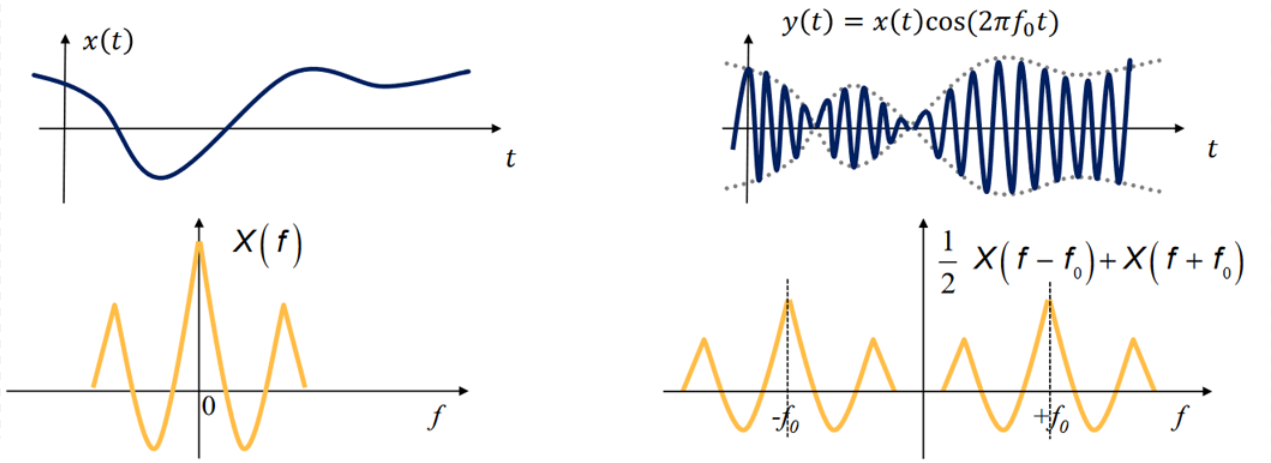
\includegraphics[width=0.8\textwidth]{img/signal modulation.png}
        \caption{Graphical representation of the modulation}
        \label{fig:Modulation}
      \end{figure}
      We can see that as a result of the modulation, the spectrum of the signal is shifted around
      the frequency $f_0$, as shown in figure \ref{fig:Modulation}.\\

    \end{subsection}
    \begin{subsection}{Signal demodulation}
      When modulating a signal, we alter it a bit, centering it around the frequency $f_0$, shifting
      the spectrum of the signal. The effect of this operation is not trivial.\\
      To recover the original signal, we need to multiply the modulated signal by a sinusoidal
      function at the same frequency $f_0$ as the one used for the modulation. This allows us to
      shift the spectrum back to the original position.\\
      This operation is called \textbf{demodulation}.\\
      A given modulated signal $Y(f)$
      \begin{equation}
        Y(f) = \frac{A}{2}[X(f-f_0) + X(f+f_0)]
      \end{equation}
      shown in figure \ref{fig:Demodulation1}
      \begin{figure}[h]
        \centering
        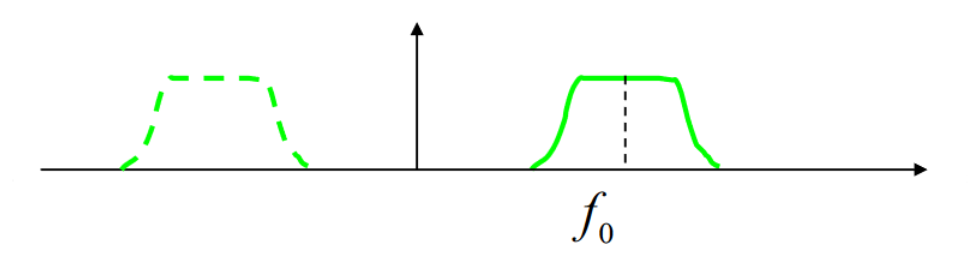
\includegraphics[width=0.8\textwidth]{img/demodulation1.png}
        \caption{A modulated signal at frequency $f_0$}
        \label{fig:Demodulation1}
      \end{figure}
      can be demodulated by multiplying it by the same sinusoidal function used for the modulation
      \begin{equation}
        Y'(f) = Y(f) \cdot cos(2\pi f_0 t)= \frac{A}{2}X(f)+\frac{A}{4}[X(f-2f_0)+X(f+2f_0)]
      \end{equation}
      shown in figure \ref{fig:Demodulation2}\\
      \begin{figure}[h]
        \centering
        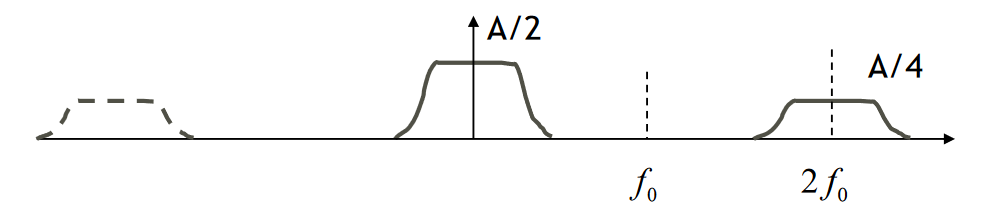
\includegraphics[width=0.8\textwidth]{img/demodulation2.png}
        \caption{A demodulated signal at frequency $f_0$}
        \label{fig:Demodulation2}
      \end{figure}
      This doesn't allow us to recover the original spectrum of the signal.
      That's why we need to use a \textbf{low-pass filter} to remove the frequency components at
      $2f_0$ and its symmetrical counterpart, as shown in figure \ref{fig:Demodulation3}.\\
      \begin{figure}[h]
        \centering
        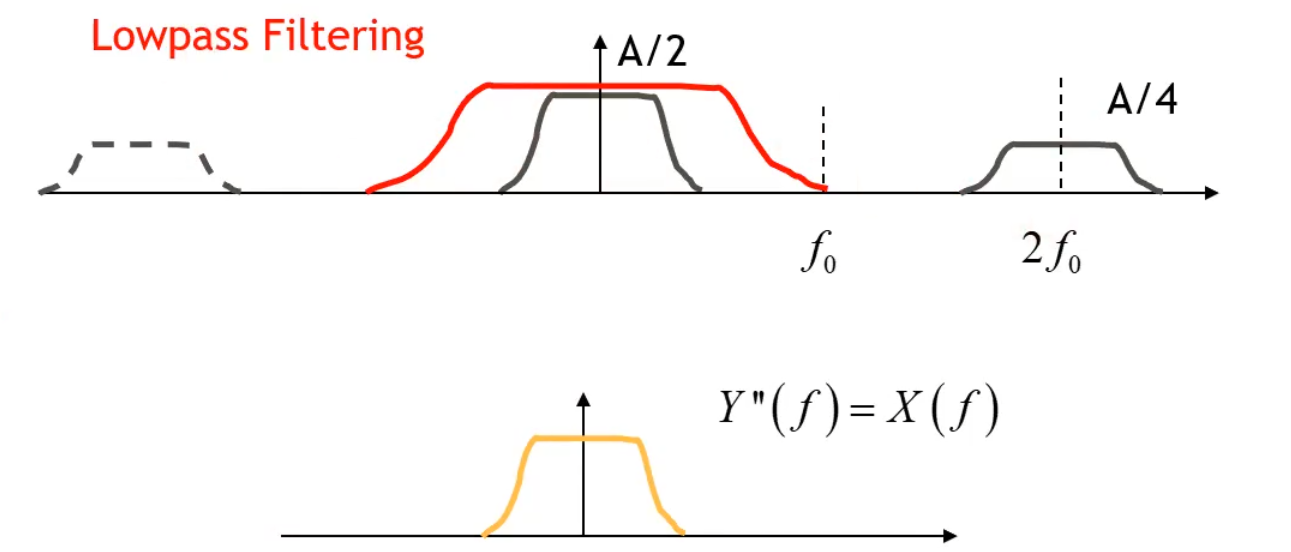
\includegraphics[width=0.8\textwidth]{img/demodulation3.png}
        \caption{A demodulated signal at frequency $f_0$ after a low-pass filter}
        \label{fig:Demodulation3}
      \end{figure}

    \end{subsection}
    \begin{subsection}{Frequency Multiplexing(FDM)}
      Modulation and demodulation allows multiple wireless communication systems to coexist at different
      frequencies.\\
      For example, if i want to transmit different signals with overlapping bandwidths, i can simply
      modulate each signal at a different frequency, and then transmit them all together, as shown in
      figure \ref{fig:FDM}.\\
      Once received the signal, each of those signals can be demodulated by multiplying it by the 
      same function at the same frequency used for the modulation.\\
      \begin{figure}[h]
        \centering
        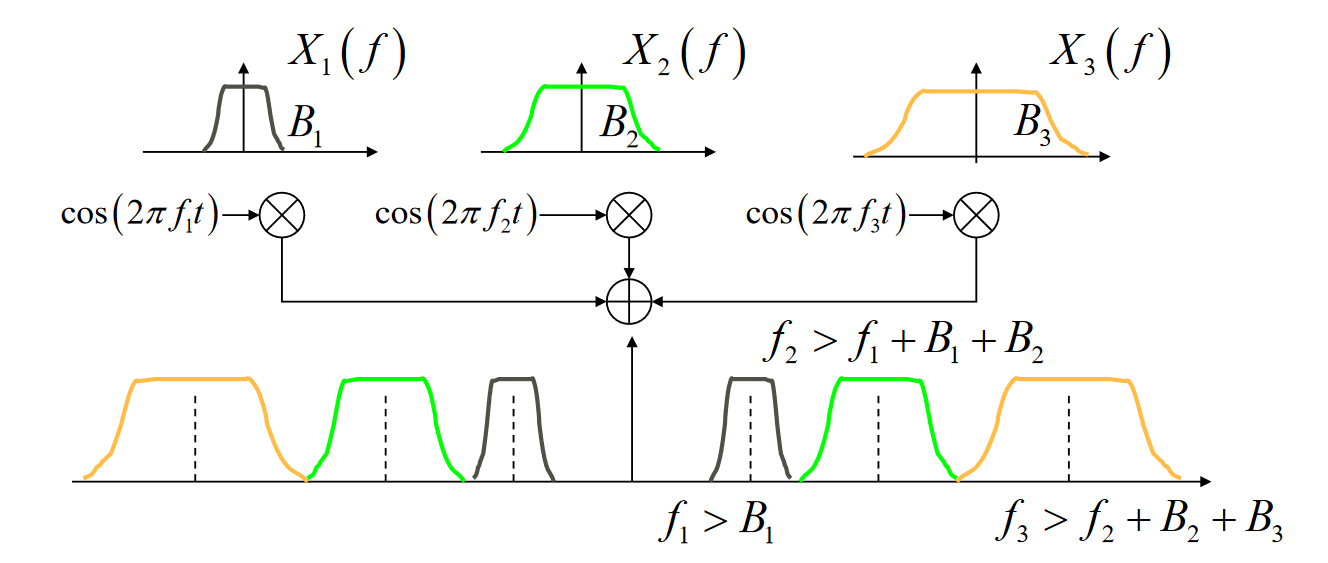
\includegraphics[width=0.9\textwidth]{img/FDM.png}
        \caption{Frequency Multiplexing}
        \label{fig:FDM}
      \end{figure}
    \end{subsection}
    \begin{subsection}{Analog-to-Digital Conversion}
      We can now deal with signals, but we still have to convey information.\\
      The informations can be both \textbf{analog} or \textbf{digital}. Usually, transmitting digital
      information is ideal, because it has some advantages, such as error detection and correction,
      and the possibility to compress the information. On the other hand, we still have to convert
      digital information to analog information to be transmitted over the channel, after converting
      it to a stream of bits.\\
      Once the signal is received, it has to be converted back to digital information. To do so,
      first of all the signal it has to be sampled, which can be a lossless operation if the sampling
      frequency is high enough.\\
      After the sampling, the sample has to be quantized, which is the process of converting the
      amplitude of the sample to a digital value at discrete times( because it is a continuous
      time function, which would require an infinite number of digits to represent). Each of those 
      values is associated with a given amplitude, which is associated to a number, which 
      eventually is converted into binary digits. We can also observe that quantization is a lossy
      operation by definition.\\
      At the end of the fair, a sequence of bits is obtained, which can be transmitted over the
      channel.\\
      \begin{figure}[h]
        \centering
        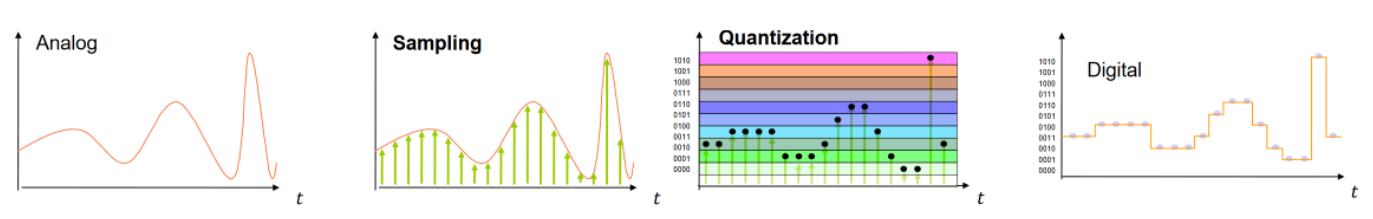
\includegraphics[width=\textwidth]{img/analog to digital.png}
        \caption{Analog-to-Digital Conversion}
        \label{fig:ADC}
      \end{figure}
      \begin{subsubsection}{Sampling theorem}
        As previously stated, the sampling operation can be lossless if the sampling frequency is
        high enough. This is because of the \textbf{Nyquist sampling theorem}, which states
        that a signal can be perfectly reconstructed from its samples if the sampling frequency is
        at least twice the bandwidth of the signal.\\
        \begin{equation}
          f_c=\frac{1}{T_c}>2B\to T_c<\frac{1}{2B}
        \end{equation}
        where $f_c$ is the sampling frequency, $T_c$ is the sampling period, and $B$ is the bandwidth.
        \end{subsubsection}
    \end{subsection}
\end{section}

\begin{section}{Signal Transmission and Reception}
  Now that we know how a signal can be represented and processed, we can start to think how each 
  component of a communication system can be designed.\\
  \begin{subsection}{Digital Modulations}
    The end goal is to have a reliable communication system, which can transmit and receive
    information. As such, a important design choose is the signal waveform to transmit.\\
    The \textbf{modulator} is the component of the system that takes the digital information and 
    modulates it to a signal that can be transmitted over the channel. The demodulator component 
    just does the opposite, taking the signal and converting it back to digital information.\\

    \begin{boxH}
      \textbf{Modulation} is the process of varying one or more properties of a periodic waveform, called
      the \textbf{carrier}, with a modulating signal that typically contains information to be
      transmitted.
    \end{boxH}
    This process is necessary not only to cope with the analog channel, but also to allow multiple
    communication systems( which means different signals) to coexist in the same channel.\\

    Generally, digital and analog modulations resort to basic modulation types:
    \begin{itemize}
      \item \textbf{Amplitude Modulation(AM)}, which changes the amplitude of the carrier
      \item \textbf{Frequency Modulation(FM)}, which changes the frequency of the carrier
      \item \textbf{Phase Modulation(PM)}, which changes the phase of the carrier
    \end{itemize}
    \begin{subsubsection}{Amplitude Modulation(AM)}
      The amplitude modulation is the simplest form of modulation.\\
      The amplitude of an high-carrier signal(like a cosine signal) is varied according to the 
      instantaneous amplitude of the modulating message signal $m(t)$.\\
    \end{subsubsection}
    \begin{subsubsection}{Frequency Modulation(FM)}
      In frequency modulation, the frequency of the carrier signal is varied by the modulating
      signal $m(t)$, while the amplitude of the carrier signal is kept constant.\\
      This means that the as the amplitude of the information signal varies, the carrier frequency
      varies as well. For example, if the amplitude of the information signal increases, the
      frequency of the carrier signal increases as well.\\
      \begin{figure}[h]
        \centering
        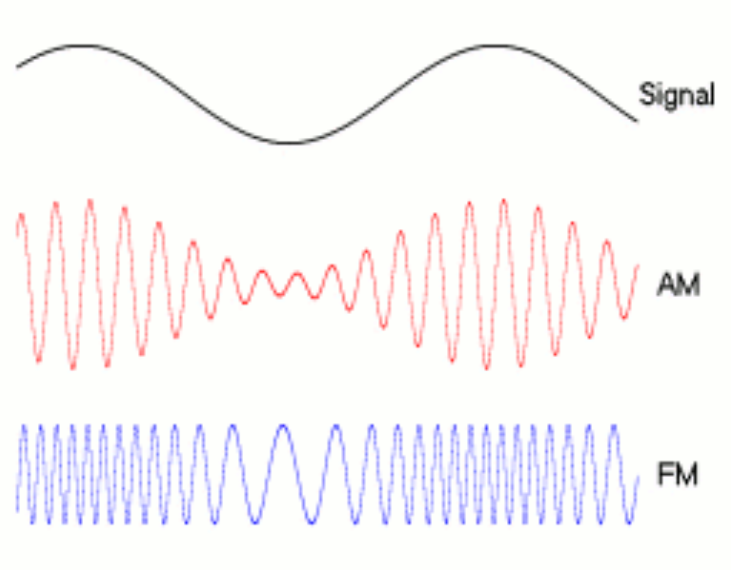
\includegraphics[width=0.4\textwidth]{img/AM-FM.png}
        \caption{An example of a signal modulated in amplitude and frequency}
        \label{fig:AM-FM}
      \end{figure}
    \end{subsubsection}
    \begin{subsubsection}{Phase Modulation(PM)}
      Phase modulation is a form of modulation that encodes the signal $m(t)$ as a variation in the
      instantaneous phase of a carrier wave.\\
      This means that the phase of a carrier is modulated to follow the changing in the signal 
      amplitude of the message signal.\\

      The peak amplitude and the frequency of the carrier signal are maintained constant, but as 
      the amplitude of the message signal changes, the phase of the carrier changes 
      correspondingly.\\
      \begin{figure}[h]
        \centering
        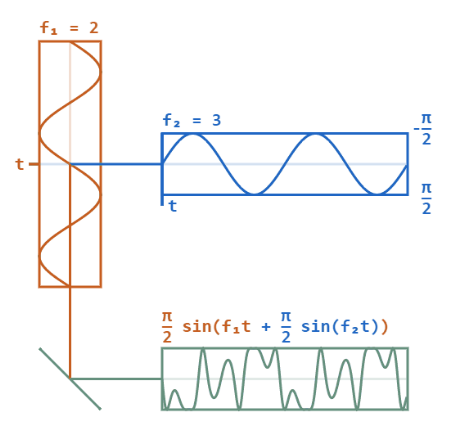
\includegraphics[width=0.5\textwidth]{img/PM.png}
        \caption{An example of a signal modulated in phase. The modulating wave(in blue) is modulating
          the phase of the carrier wave(in red), resulting in the PM signal(in green)}
        \label{fig:PM}
      \end{figure}
    \end{subsubsection}
    \begin{subsubsection}{Analog-to-Digital modulations}
      Even if the world has turned to digital, transmitted signals are analog.\\
      This means that the digital information has to be converted to an analog signal to be
      transmitted over the channel. But the receiver still need to understand the digital information
      from the received signal.\\
      To be sure that the information can be recovered, the signal has to be modulated in a way that
      the receiver can understand the digital information. This can be done by varying some proprieties
      of the carrier signal, such as the amplitude, the frequency, or the phase, to represent the
      digital information.\\
      \begin{figure}[h]
        \centering
        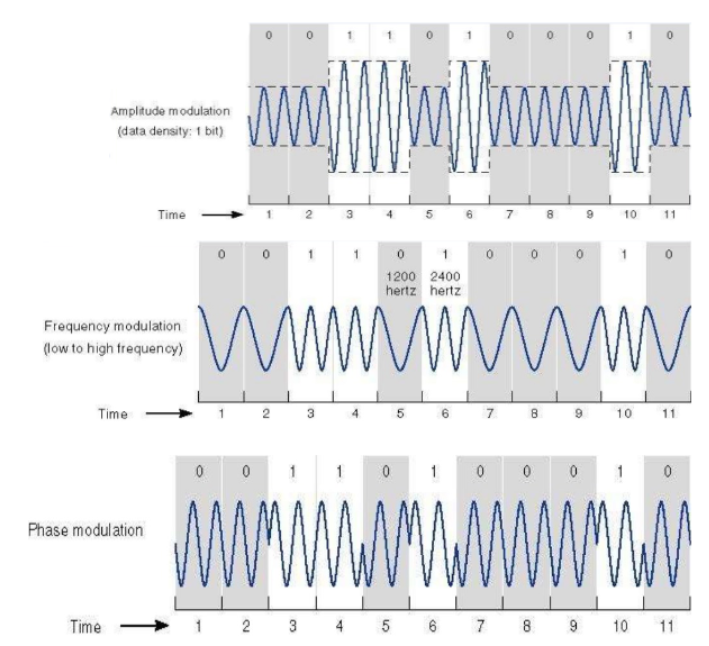
\includegraphics[width=0.5\textwidth]{img/modulation encoding.png}
        \caption{Some example of modulations used to represent digital information. From top to bottom:
          Amplitude Shift Keying, Frequency Shift Keying, Phase Shift Keying}
        \label{fig:DigitalModulation}
      \end{figure}
      The carrier signal is used to modulate the digital information, so we can distinguish between
      different kinds of signals:
      \begin{itemize}
        \item the \textbf{the baseband signal}, which is the unmodulated signal, whose spectrum is
          centered around zero frequency
        \item the \textbf{passband signal}, which is the modulated signal, whose spectrum is centered
          around the carrier frequency
      \end{itemize}
      The baseband signal can be converted to a passband signal by multiplying it by a carrier signal
      with the desired frequency.\\
    \end{subsubsection}
    \begin{subsubsection}{Baseband Signals}
      The simplest kind of digital modulation is the \textbf{Pulse Amplitude Modulation(PAM)}, which
      is a form of modulation where the message signal is encoded in the amplitude of a series of
      signal pulses.\\
      For example, if we have a binary signal, we can encode the 0 as a low amplitude pulse $-A$, and the
      1 as a high amplitude pulse $A$. The simplest pulse is a rectangular one, but other kind of 
      pulses can be used.\\
      If we have a binary PAM(2-PAM), the signal can be represented as:
      \begin{itemize}
        \item $s(t)=g(t) \to "1"$
        \item $s(t)=-g(t) \to "0"$
      \end{itemize}
      where $g(t)$ is the basic pulse shape.\\
      \begin{figure}[h]
        \centering
        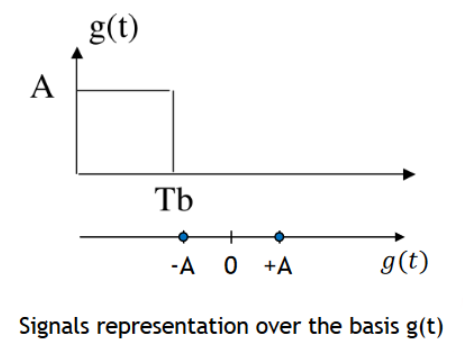
\includegraphics[width=0.4\textwidth]{img/2-PAM.png}
        \caption{An example of a 2-PAM signal representation}
        \label{fig:PAM}
      \end{figure}
    \end{subsubsection}
    \begin{subsubsection}{M-ary PAM}
      WA 2-PAM signal can only represent 1 bit of information. To represent more bits, we can use
      M-ary PAM, where M is the number of different symbols that can be represented, while still
      using the same base signal.\\
      For example, a 4-PAM signal can represent 2 bits of information by defining 4 levels of
      amplitude, and can be represented as:
      \begin{itemize}
        \item $s(t)=3g(t) \to "00"$
        \item $s(t)=g(t) \to "01"$
        \item $s(t)=-g(t) \to "10"$
        \item $s(t)=-3g(t) \to "11"$
      \end{itemize}
      This definition can be generalized to:
      \begin{equation}
        s_i(t)=A_i g(t),\quad i=1,2,\dots,M
      \end{equation}
      allowing to represent $log_2(M)$ bits of information.\\
      \begin{figure}[h]
        \centering
        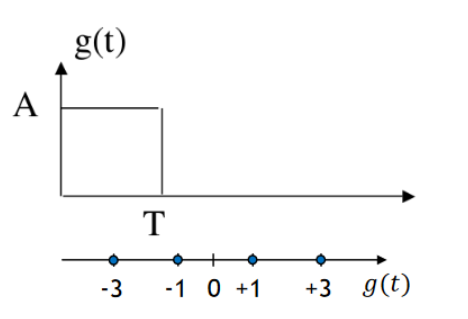
\includegraphics[width=0.4\textwidth]{img/M-PAM.png}
        \caption{An example of a 4-PAM signal representation}
        \label{fig:4-PAM}
      \end{figure}
    \end{subsubsection}
    \begin{subsubsection}{Gray Coding}
      When using M-ary PAM, it is important to use a coding that minimizes the error probability.
      After all, Symbols that are close to each other in the signal space are more likely to be 
      confused, so the choice of the number of symbols and the distance between them is 
      important.\\
      \begin{boxH}
        \textbf{Gray coding} is a strategy to \textbf{mapping bits to symbols} that minimizes the
        probability of error.
      \end{boxH}
      Gray coding achieves 1-bit error correction, meaning that if a error is to occur, it will only
      affect 1 bit of the message with a high probability.\\
      \begin{figure}[h]
        \centering
        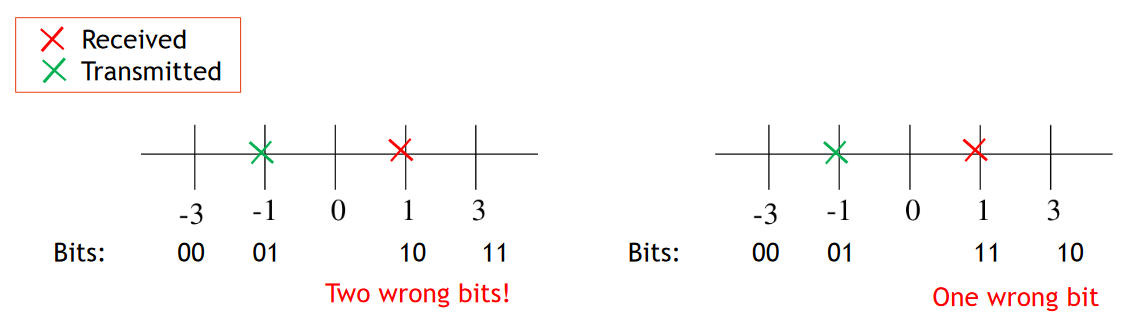
\includegraphics[width=0.8\textwidth]{img/gray coding.png}
        \caption{An example of a 4-PAM signal representation using Gray coding}
        \label{fig:GrayCode}
      \end{figure}
    \end{subsubsection}
    \begin{subsubsection}{Energy per bit}
      A measure of the energy efficiency of a modulation can be obtained by calculating the avarage
      energy per bit.\\
      The energy per bit can be defined as 
      \begin{equation}
        E_b=\frac{E_s}{log_2(M)}
      \end{equation}
      where $E_s$ is the energy of the signal, and $M$ is the number of symbols, or in a more
      discursive way, the average energy per symbol divided by the number of bits carried by 
      each symbol.\\
      The energy per symbol can be calculated as
      \begin{equation}
        E_s=\int_{0}^{T} (S_m(t))^2 dt= (A_m)^2 \int_{0}^{T} (g(t))^2 dt= (A_m)^2 E_g
      \end{equation}
      where $S_m(t)$ is the modulated signal, $A_m$ is the amplitude of the modulated signal, $g(t)$
      is the base pulse, and $E_g$ is the energy of the base pulse.\\

      For example, the average energy per symbol for the 4-PAM of figure \ref{fig:4-PAM} is
      \begin{equation}
        E_s=\frac{3^2T+1^2T+1^2T+3^2T}{4}=5T
      \end{equation}
      \begin{subsubsection}{Bandpass Signals}
        As previously stated, to transmit a baseband signal $s(t)$ trough a passband channel, we 
        have to modulate it at a certain frequency $f_c$, by multiplying it by a sinusoidal carrier
        signal with that frequency, otherwise it will be centered around zero frequency.\\
      \end{subsubsection}
      \begin{subsubsection}{Bandwidth Occupancy}
        \end{subsubsection}

    \end{subsubsection}


    
  \end{subsection}
\end{section}
